In this chapter we will show the simulations conducted to evaluate the consensus algorithm.

\begin{figure}
\centering
\includegraphics[width=0.8\textwidth]{chapters/chapter-04/figures/iris_model.png}
\caption{Iris model}
\label{fig:iris_model}
\end{figure}

As said in the Chapter \ref{chap:system_architecture}, the software used is Gazebo.
We ran SITL (Software in the loop) simulations, through the utilities provided by
the PX4 firmware. It provides models of the main topologies of aerial vehicles,
such as plane, VTOL, Tailsitter VTOL and quadrotor.
We will use the quadrotor model called Iris, which is shown in the picture \ref{fig:iris_model}.

The PX4 firmware is run on a simulated hardware and all the ROS nodes are executed
on the same computer. The physics is simulated by Gazebo and all the components
are interfaced through Gazebo plugins. In this way, the model can interact with
all the external simulated components.

The Gazebo model is specified, using SDF language, in a Gazebo model file and
the dynamic parameters are listed in it and the geometry
is included as well.

The simulations that we will show are of three kinds. Firstly, we will present only
the trajectory following problem of a formation of two drones.
Secondly, we will send a disturbance to one of the drones and we will stop it
in its position. Thirdly, we will introduce a disturbance which will make one of the drones
go back following its trajectory backward.
We see how the consensus algorithm reacts to these disturbances and forces the other
drone to preserve the formation.
Although only two drones have been used because of the computational load of the simulation, but the
concept can be extended freely to an arbitrary number of drones.

\section{Trajectory following}

In the simulation two drones have been used. The trajectory of the mission is shown
in \ref{fig:trajectory}.

\begin{figure}
\centering
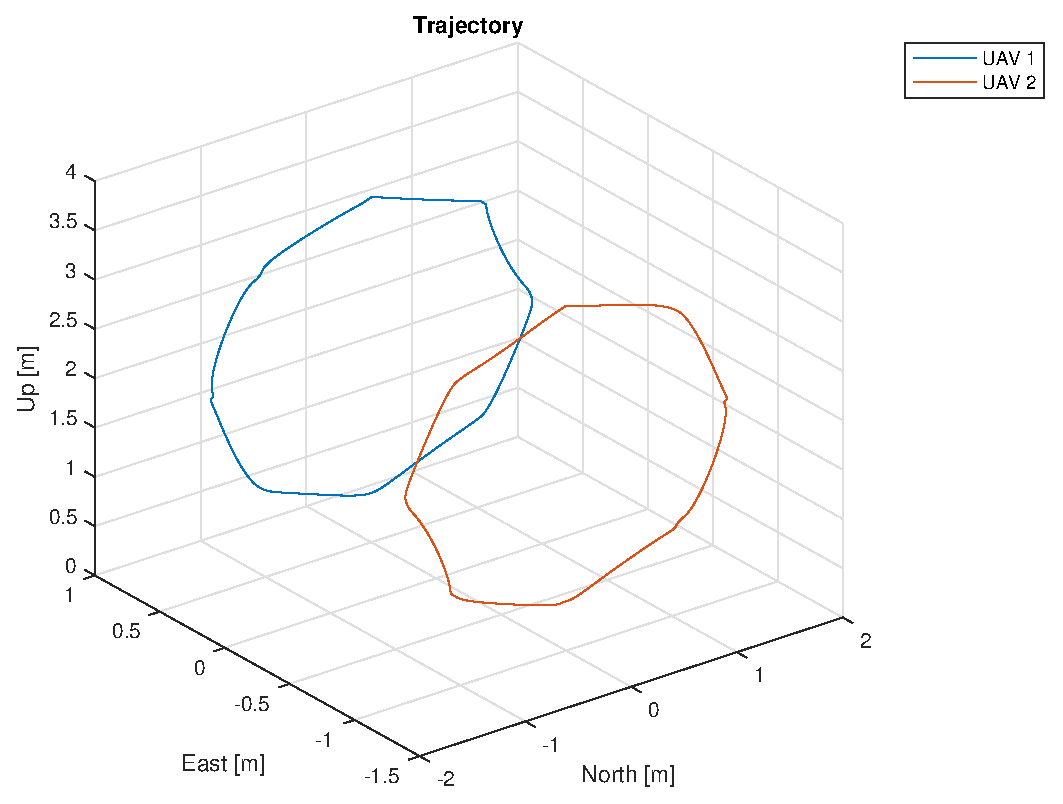
\includegraphics[width=0.7\textwidth]{chapters/chapter-04/figures/trajectory.eps}
\caption{Trajectory}
\label{fig:trajectory}
\end{figure}

Both drones start in the upper point of their circle and then they move along the
trajectory in opposite directions. The mission terminates when both drones reach
their starting point.
The evolution of the trajectory in time of the first drone can be seen in the Figure
\ref{fig:trajectory_during_time}.

\begin{figure}
\centering
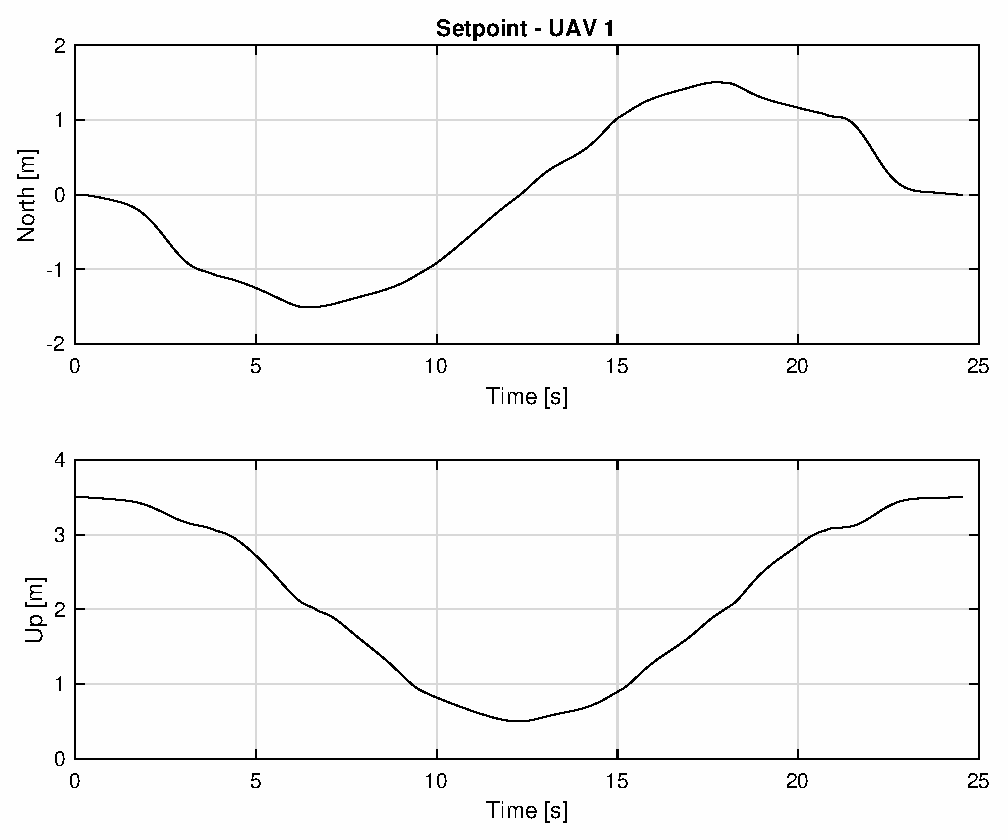
\includegraphics[width=0.7\textwidth]{chapters/chapter-04/figures/pos.eps}
\caption{Evolution of the trajectory in time of the first drone}
\label{fig:trajectory_during_time}
\end{figure}

How the two drones follow their trajectory is shown in the Figures
\ref{fig:following_1} and \ref{fig:following_2}.

\begin{figure}
\centering
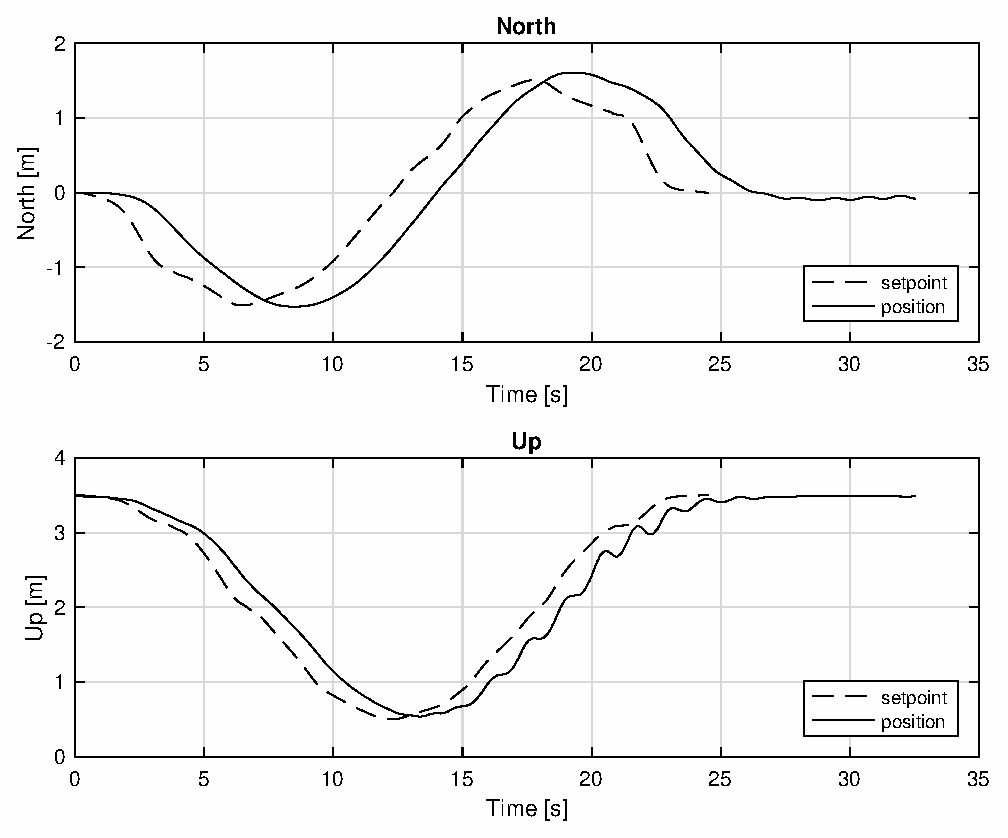
\includegraphics[width=0.7\linewidth]{chapters/chapter-04/figures/following_1.eps}
\caption{Target following drone 1}
\label{fig:following_1}
\end{figure}

\begin{figure}
\centering
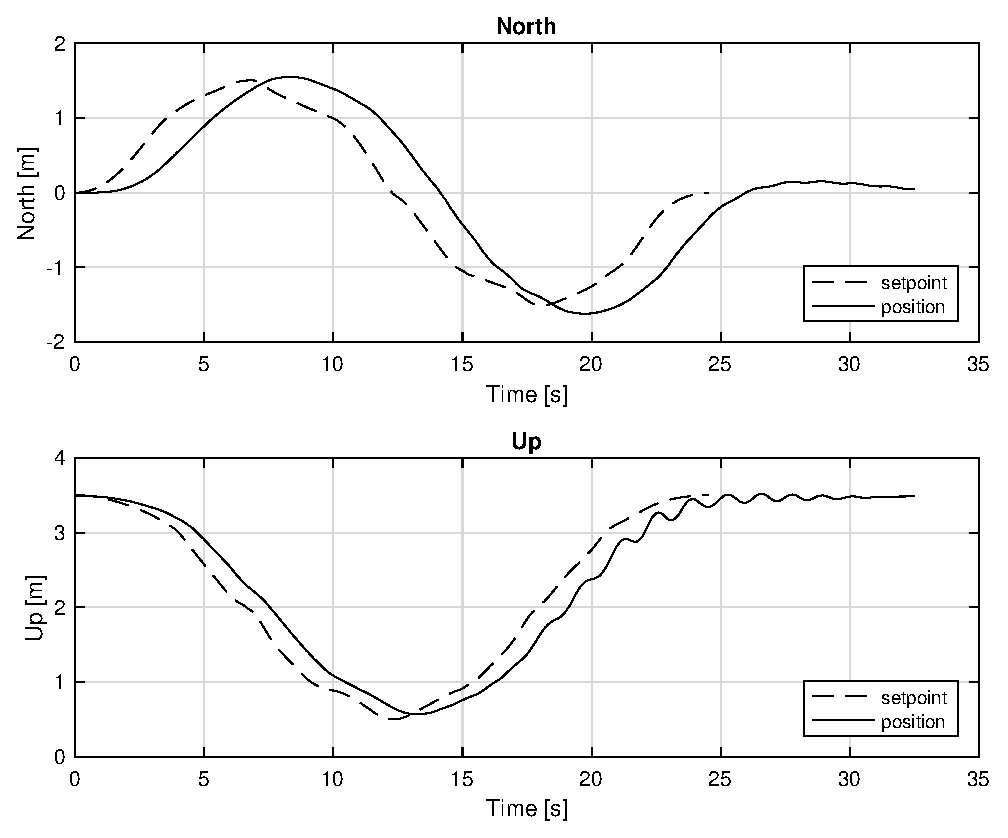
\includegraphics[width=0.7\linewidth]{chapters/chapter-04/figures/following_2.eps}
\caption{Target following drone 2}
\label{fig:following_2}
\end{figure}

There are some delays due to the fact that the autopilot needs time to follow the target,
but the drones can follow if successfully.
In fact, they arrive at their final position at the same time.

\begin{figure}
\centering
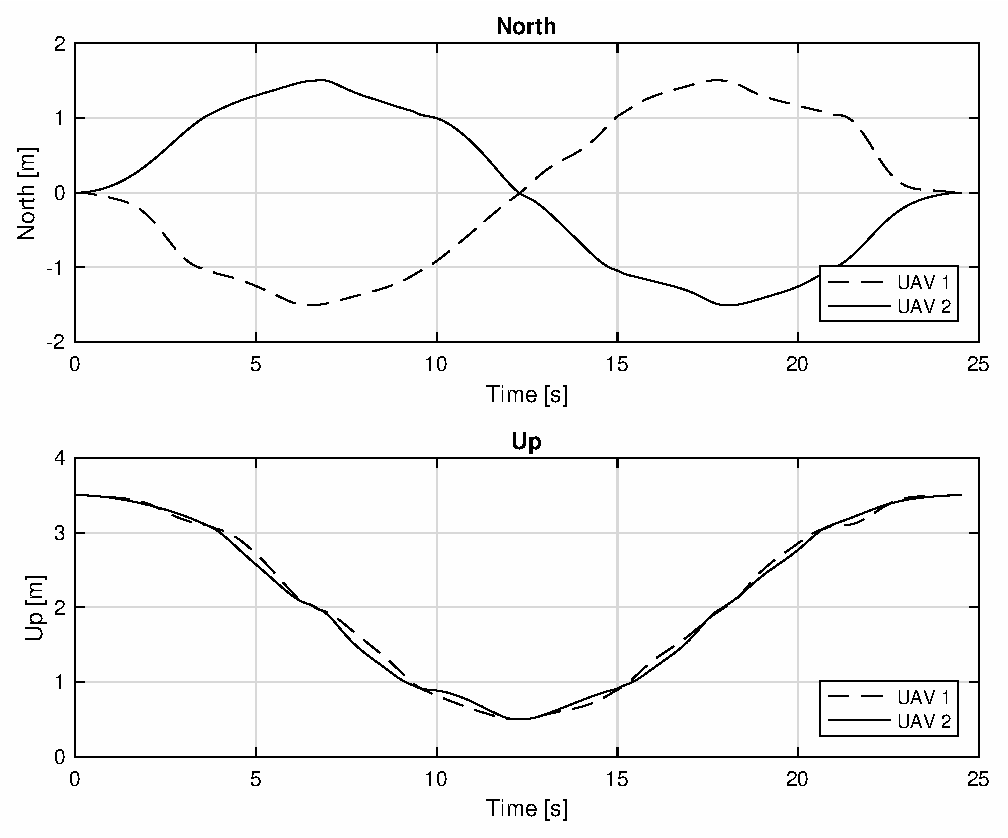
\includegraphics[width=0.7\textwidth]{chapters/chapter-04/figures/overlapped.eps}
\caption{Positions of the two drones in time}
\label{fig:overlapped}
\end{figure}

If we also consider the Figure \ref{fig:overlapped}, we can see that both drones
are synchronized during the execution of the mission. In the next cases, we will
add disturbances in order to make the effects of the algorithm more evident.


\section{First disturbance}
In this scenario, we use the same trajectory as before (Figure \ref{fig:trajectory}),
but in this case we stop one of the two drones and the other will follow it.
The Figure \ref{fig:disturbance} shows the disturbance applied to the first drone at time 11s.

\begin{figure}
\centering
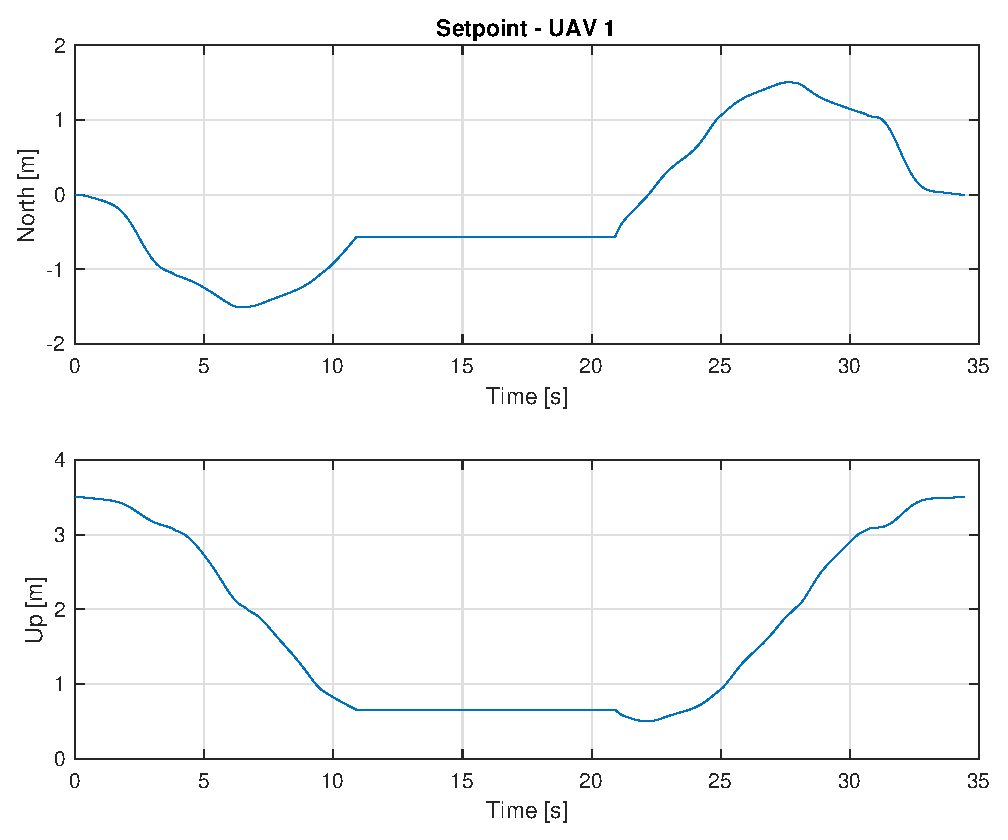
\includegraphics[width=0.7\textwidth]{chapters/chapter-04/figures/pos_1.eps}
\caption{Disturbance}
\label{fig:disturbance}
\end{figure}

We can now see how the two drones execute the mission. The second drone tries to
go on when the first is interrupted, but then the consensus stops it. The plots are
shown in the Figures \ref{fig:following_1_1} and \ref{fig:following_2_1}.

\begin{figure}
\centering
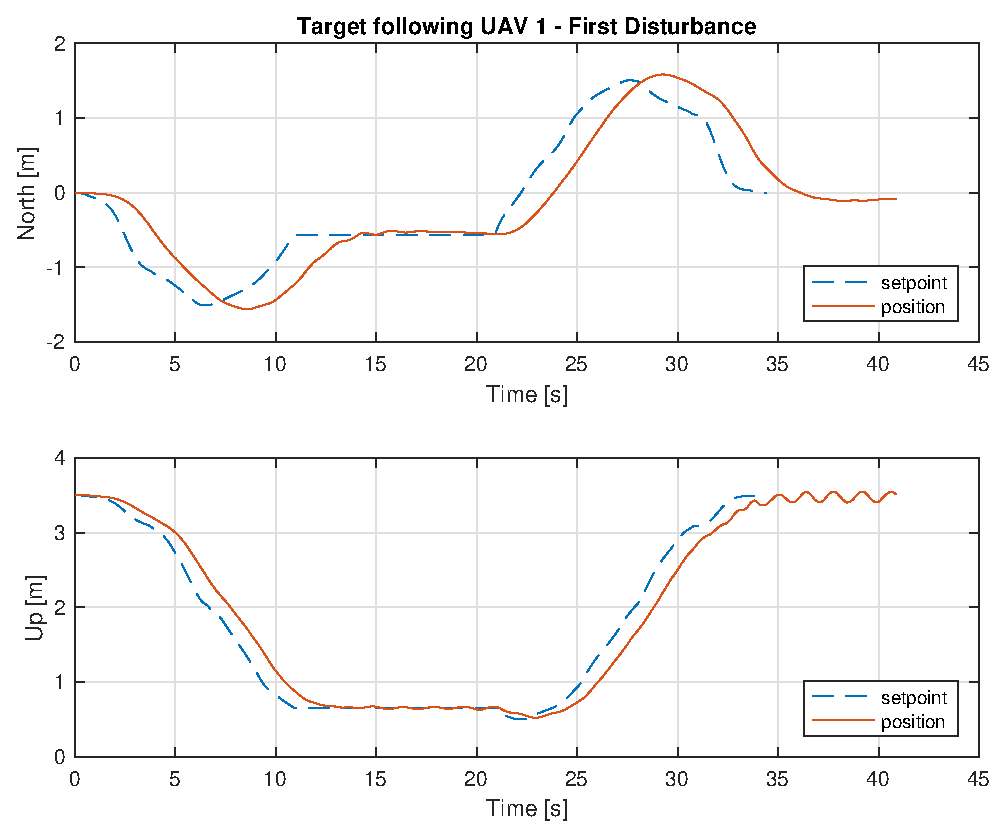
\includegraphics[width=0.7\linewidth]{chapters/chapter-04/figures/following_1_1.eps}
\caption{Target following drone 1}
\label{fig:following_1_1}
\end{figure}

\begin{figure}
\centering
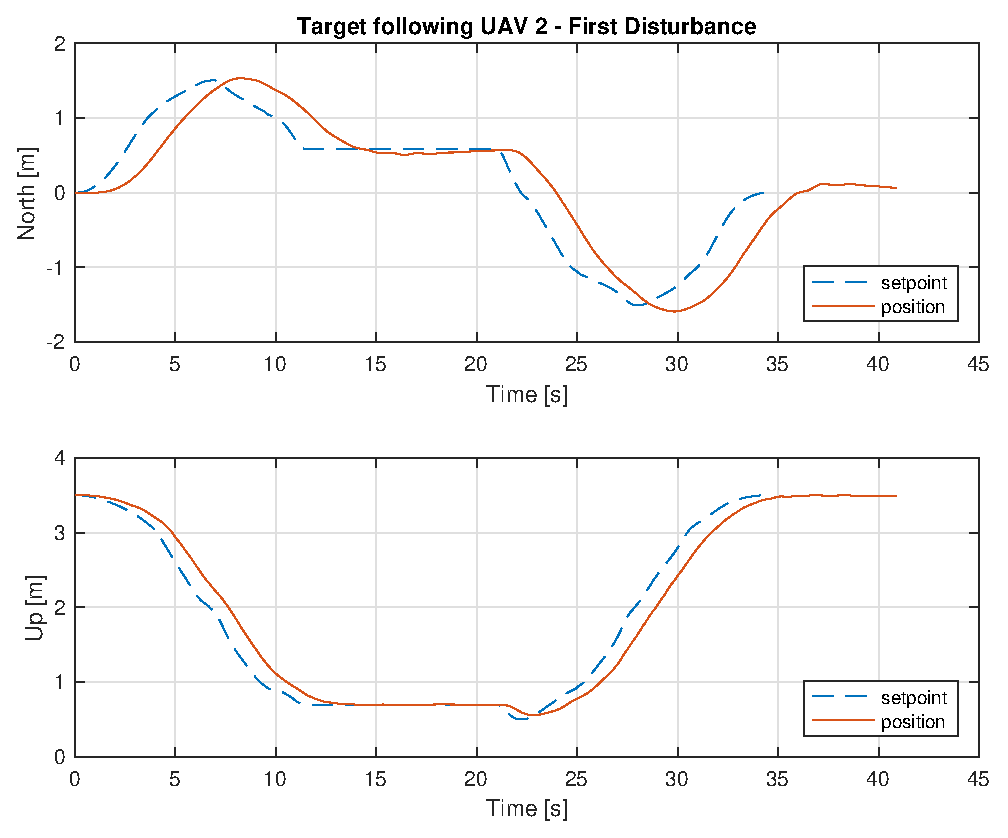
\includegraphics[width=0.7\linewidth]{chapters/chapter-04/figures/following_2_1.eps}
\caption{Target following drone 2}
\label{fig:following_2_1}
\end{figure}

Finally, the Figure \ref{fig:overlapped_1} is a graph representing the overlapped
positions of the two drones.


\begin{figure}
\centering
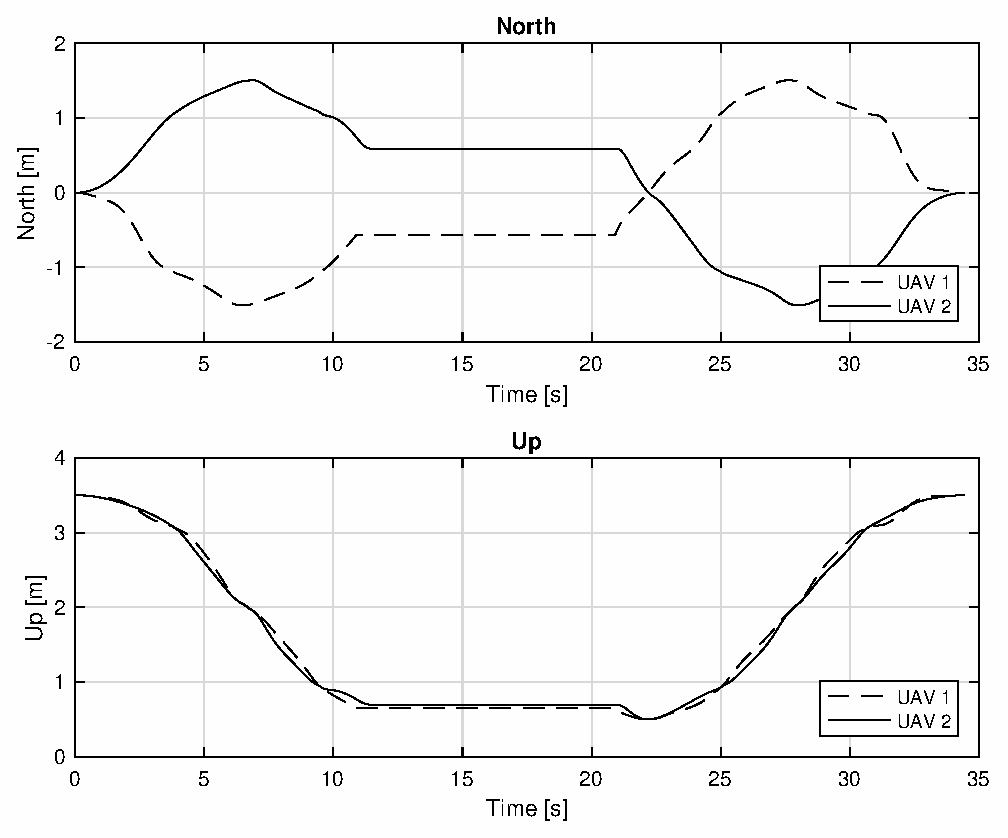
\includegraphics[width=0.7\textwidth]{chapters/chapter-04/figures/overlapped_1.eps}
\caption{Positions of the two drones in time}
\label{fig:overlapped_1}
\end{figure}


\section{Second disturbance}
The trajectory used is always the same (Figure \ref{fig:trajectory}), but this time
the disturbance is different. Now we force one drone to go back through the trajectory
which has travelled so far.
After the disturbance, the drone can resume the trajectory and complete the mission.
We can see the effect of the disturbance on the trajectory in the Figure \ref{fig:disturbance_2}.

\begin{figure}
\centering
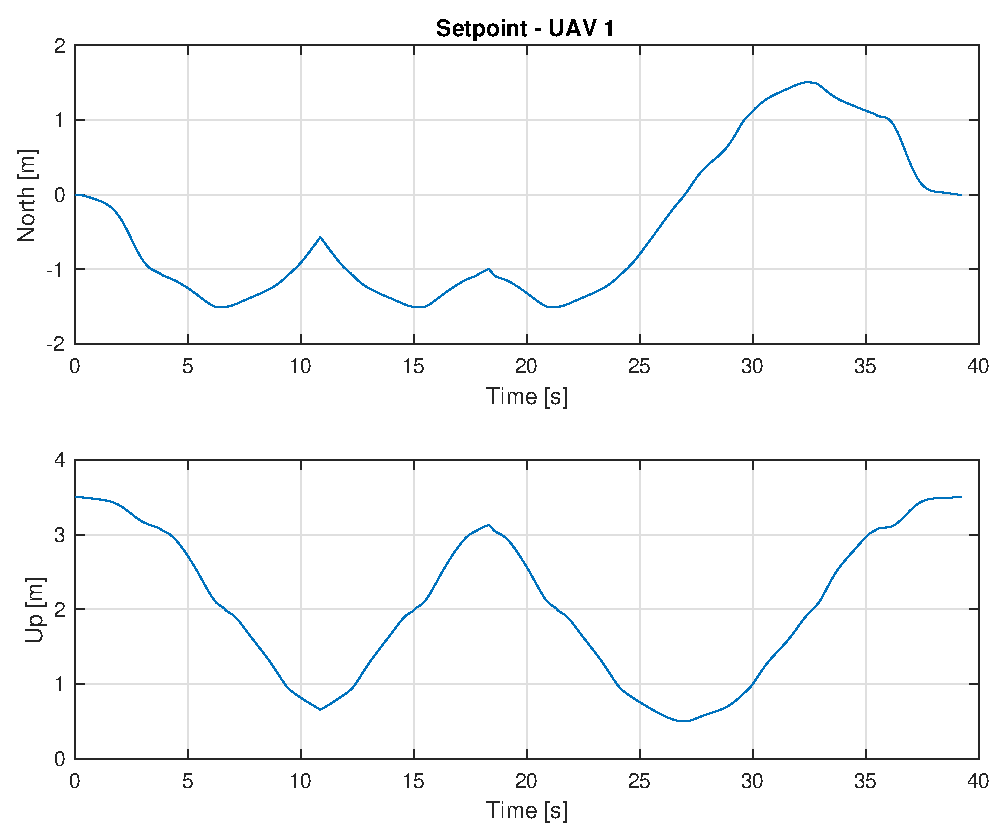
\includegraphics[width=0.7\textwidth]{chapters/chapter-04/figures/pos_2.eps}
\caption{Disturbance}
\label{fig:disturbance_2}
\end{figure}

At time 11s the disturbance starts and the drone begins to go back. At time 26s,
the drone has returned to the position where the disturbance is started.

In this situation, the other drone recognizes that the other machine is going backward
for an unknown reason and starts to follow it. We can see how the mission is done
by the two drones in the Figures \ref{fig:following_1_2} and \ref{fig:following_2_2}.

\begin{figure}
\centering
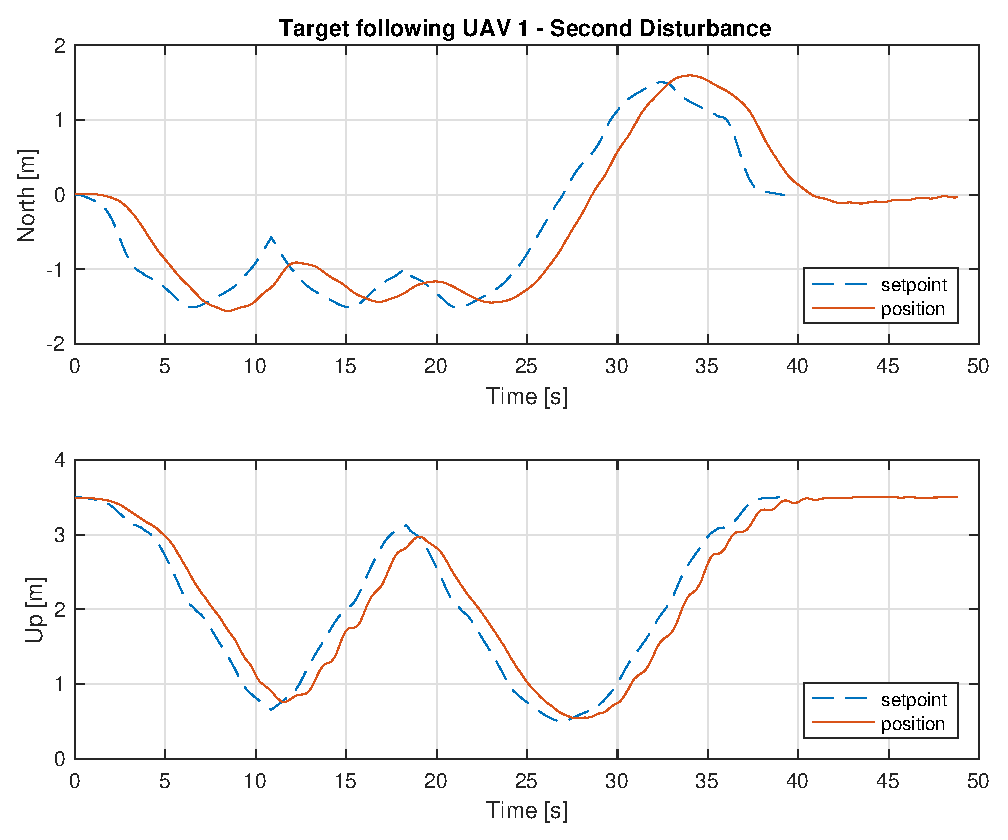
\includegraphics[width=0.7\linewidth]{chapters/chapter-04/figures/following_1_2.eps}
\caption{Target following drone 1}
\label{fig:following_1_2}
\end{figure}

\begin{figure}
\centering
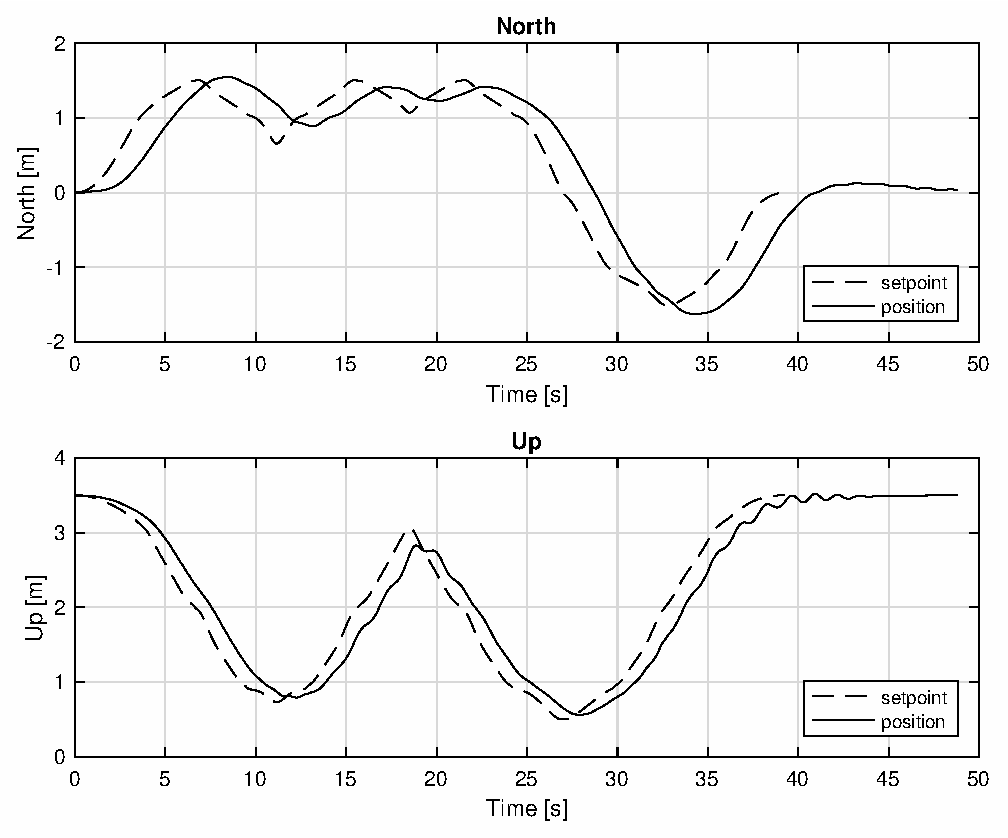
\includegraphics[width=0.7\linewidth]{chapters/chapter-04/figures/following_2_2.eps}
\caption{Target following drone 2}
\label{fig:following_2_2}
\end{figure}

\begin{figure}
\centering
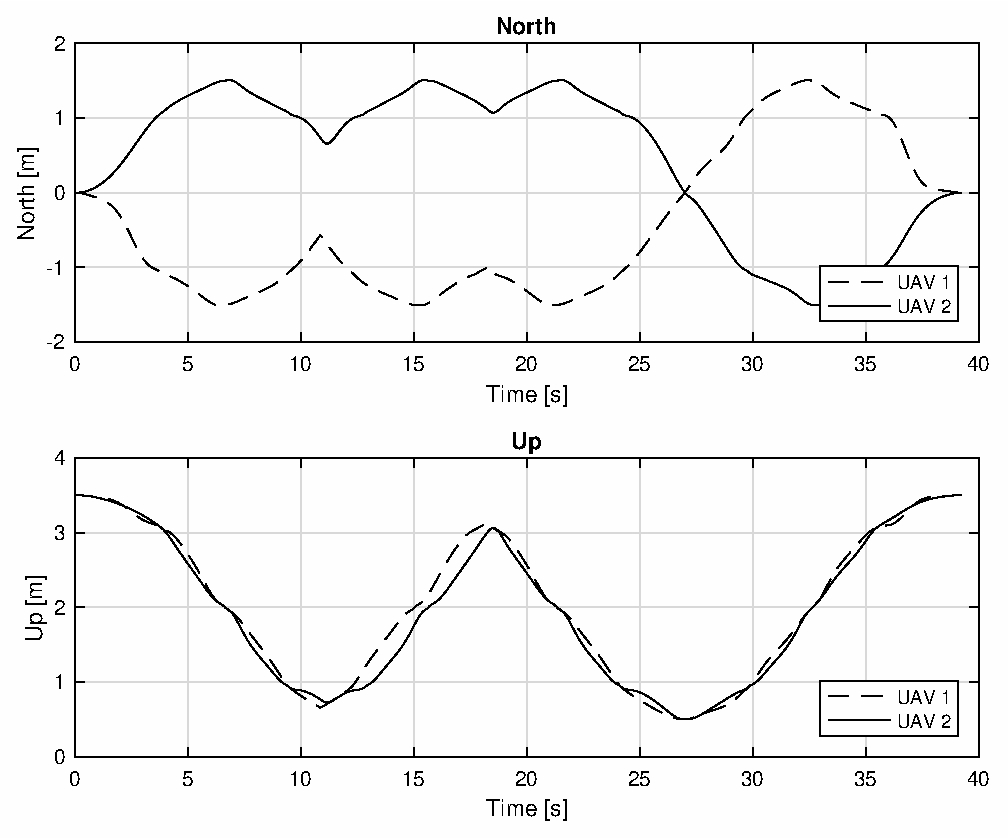
\includegraphics[width=0.7\textwidth]{chapters/chapter-04/figures/overlapped_2.eps}
\caption{Positions of the two drones in time}
\label{fig:overlapped_2}
\end{figure}


Finally, the Figure \ref{fig:overlapped_2}, is a graph representing the overlapped
positions of the two drones.
